\chapter{Graph Construction}
\label{chap:graph_construction}

A fundamental prerequisite for applying Graph Neural Networks (GNNs) is the existence of a relational topology. Unlike spatial domains such as traffic or energy grids—where physical proximity dictates connectivity, retail product assortments lack a naturally occurring, dynamic structural graph. While static product hierarchies (e.g., categories and departments) exist, they are often too rigid to capture the complex, time-varying correlations driven by substitution effects, complementarity, and promotional events. Consequently, to fully leverage spatial message-passing architectures, the relational structure between products must be explicitly inferred from their historical demand signals.

This chapter details the data-driven methodologies developed to construct these evolving product graphs. Section \ref{sec:dynamic_graph_init} formalizes the dynamic graph initialization process, establishing how temporal sliding windows and sparsity thresholds are utilized to capture transient market dynamics while strictly preventing data leakage. Building upon this foundation, the subsequent sections evaluate the two distinct mathematical approaches used to evaluate product similarity and instantiate the graph edges: Spearman rank correlation (Section \ref{subsec:spearman_graphs}), which captures monotonic co-movement, and \ac{CID} (Section \ref{subsec:cid_graphs}), which connects products based on their structural volatility and demand shape.

\section{Dynamic Graph Initialization via Sliding Windows}
\label{sec:dynamic_graph_init}

To address the computational bottlenecks associated with fully connected $\mathcal{O}(N^2)$ graph learning in large retail catalogs, this methodology employs sparse, dynamically constructed adjacency matrices. Rather than relying on a static, predefined product hierarchy or learning a dense continuous matrix entirely from scratch during the forecasting pipeline, the ego-graph topology for each target product is explicitly initialized using a metric-based edge construction applied over sliding temporal windows.

This approach ensures that the relational structure between products adapts to shifting market dynamics, capturing transient dependencies such as seasonal correlations or co-promotional effects without suffering from data leakage. For a given time step $t$, the edge weight between a product $i$ and a neighboring product $j$ is calculated based on their historical sales series within a sliding lookback window of width $W=30$. 

To guarantee computational scalability and ensure the subsequent graph neural networks focus only on the most significant relationships, an empirical sparsity threshold ($\tau$) is applied. Depending on whether a similarity metric (e.g., Spearman correlation) or a distance metric (e.g., Complexity Invariant Distance) is utilized, the explicit dynamic adjacency matrix $A^{(t)}$ at time $t$ is formally defined as:

\begin{equation}
A_{i,j}^{(t)} = 
\begin{cases} 
1 & \text{if metric}\left(\mathbf{x}_i^{(t-W:t)}, \mathbf{x}_j^{(t-W:t)}\right) \text{ satisfies } \tau \\ 
0 & \text{otherwise} 
\end{cases}
\end{equation}

Where:
\begin{itemize}
    \item $A_{i,j}^{(t)}$ represents the explicit unweighted edge between product $i$ and $j$ for the current sliding window. (Note: continuous edge weights can also be derived directly from the metric scores).
    \item $\mathbf{x}_i^{(t-W:t)}$ is the time series data for product $i$ over the window $W$.
    \item $\text{metric}(\cdot)$ denotes the chosen pairwise evaluation function (Similarity or Distance).
    \item $\tau$ is the predefined threshold controlling the sparsity of the graph.
\end{itemize}

By thresholding these scores, the resulting ego-graphs remain sparse. This significantly reduces the memory footprint of spatial message-passing layers while firmly rooting the graph's structural evolution in observable, real-world retail correlations. The following sections detail the specific distributions and threshold selections for the two primary metrics evaluated in this study: Spearman correlation and \ac{CID}.
\section{Spearman}
\label{subsec:spearman_graphs}

\subsection{Node and Edge Distribution}
\label{subsubsec:spearman_node_edge_distribution}

The Spearman correlation was used as a similarity criterion to construct dynamic 
product graphs. In this setting, the objective is not to connect products with
similar absolute sales volumes, but rather products whose demand evolves with a
similar relative ordering within each temporal window. This is particularly
relevant in retail demand forecasting, since two products may operate at very
different sales scales while still exhibiting comparable short-term demand
movements.

\begin{figure}
    \centering
    
\includegraphics[width=0.8\linewidth]{figures/hist_focal_vs_full_spearman_similarity_W30_S1_top1pct.png}
    \caption{Histogram plot of top-1\% best Spearman similarities collected from all windows, from all possible pairs between the 60 selected products}
    \label{fig:Focal vs full}
\end{figure}


To provide guidance for selecting a threshold, the full pairwise Spearman similarity distribution was calculated on a per-sliding window basis, and each of the 60 benchmark products was compared against the entire product catalog. As shown in Figure ~\ref{fig:spearman_focal_vs_full_top1pct}, the vast majority of product pairs have very low levels of similarity (i.e., the majority of the distribution falls below 0.4), indicating that most products do not have correlated demand behaviors in any given 30 day window. The distribution is highly skewed to the right, as indicated by the thin, extended tail of high similarity values.

The tail of the distribution represents those few product pairs that demonstrate true monotonic co-movement and are therefore the only reasonable candidates for the graph's edges. Rather than choosing an arbitrary threshold, a single empirically derived threshold was derived from this tail. The top one percent of all pairwise similarities were first identified and aggregated over all time windows. The upper tail of this portion of the distribution starts approximately at $\tau_{\text{1\%}}= 0.574 $. A threshold was selected based on the mean similarity of the top-1% group:

\begin{align}
  \tau &= 0.634
\end{align}

Therefore, this threshold retains only those pairs with monotonic co-movement greater than $99 \%$ of all products in the catalog. Furthermore, instead of using the bottom edge of the tail ($\tau_{\text{1\%}}$) to anchor the threshold, this approach uses the center of mass of the tail so that weak borderline associations just above $\tau_{\text{1\%}}$ are excluded. By adopting a single objective threshold, the arbitrariness associated with evaluating multiple hand-chosen thresholds is eliminated, as well as the ambiguity regarding the number of edges in the downstream graph configuration.

Figure~\ref{fig:mean_nodes_per_window_spearman} shows the mean number of nodes
per sliding window across the 60 benchmark products at the selected threshold
$\tau = 0.634$.

To better appreciate how the time-varying patterns for the product network derived from Spearman's rank correlation coefficient evolve over time, the mean size of neighborhood evolution was evaluated across all 30-day sliding window times. The figure below clearly illustrates that the connectivity of the networks exhibits very different event-based behaviors as well as a high level of synchrony. The first and largest observed increase in overall network connectivity occurred in early 2021, with a significant spike in the mean number of connected nodes peaking above 35 in March-April 2021. These results suggest that the observed large-scale synchronized monotonic increases in rank movements for the majority of the catalogue were likely due to either a major platform-wide macro-event, a significant transition associated with the Spring Seasonal, or an aggressive marketing promotion. A subsequent drop-off in connectivity, followed by stabilization at a lower baseline (i.e., approximately five connected nodes), occurred throughout the late Summer and Early Autumn Months. In addition to these longer-duration trends, there are several smaller-duration upward blips in connectivity that can be seen at year-end holidays. In addition to a first, relatively modest sustained peak around Thanksgiving, a second, significantly higher sustained peak occurred around the time of Christmas, continuing through the early part of January 2022. These examples show how many products exhibit synchronous increases in their levels of demand simultaneously and therefore have similar movements in their sales rankings. This demonstrates again how good the Spearman method will be at identifying correlations in the movement of the sales rank of multiple products as the \( \tau = .634\) Spearman correlation measure also indicates that while the short-term structure of demand for each product may vary greatly and be potentially highly volatile during the holiday season, it follows a similar overall path in response to these external retail-related events.
\begin{figure}[htbp]
    \centering
    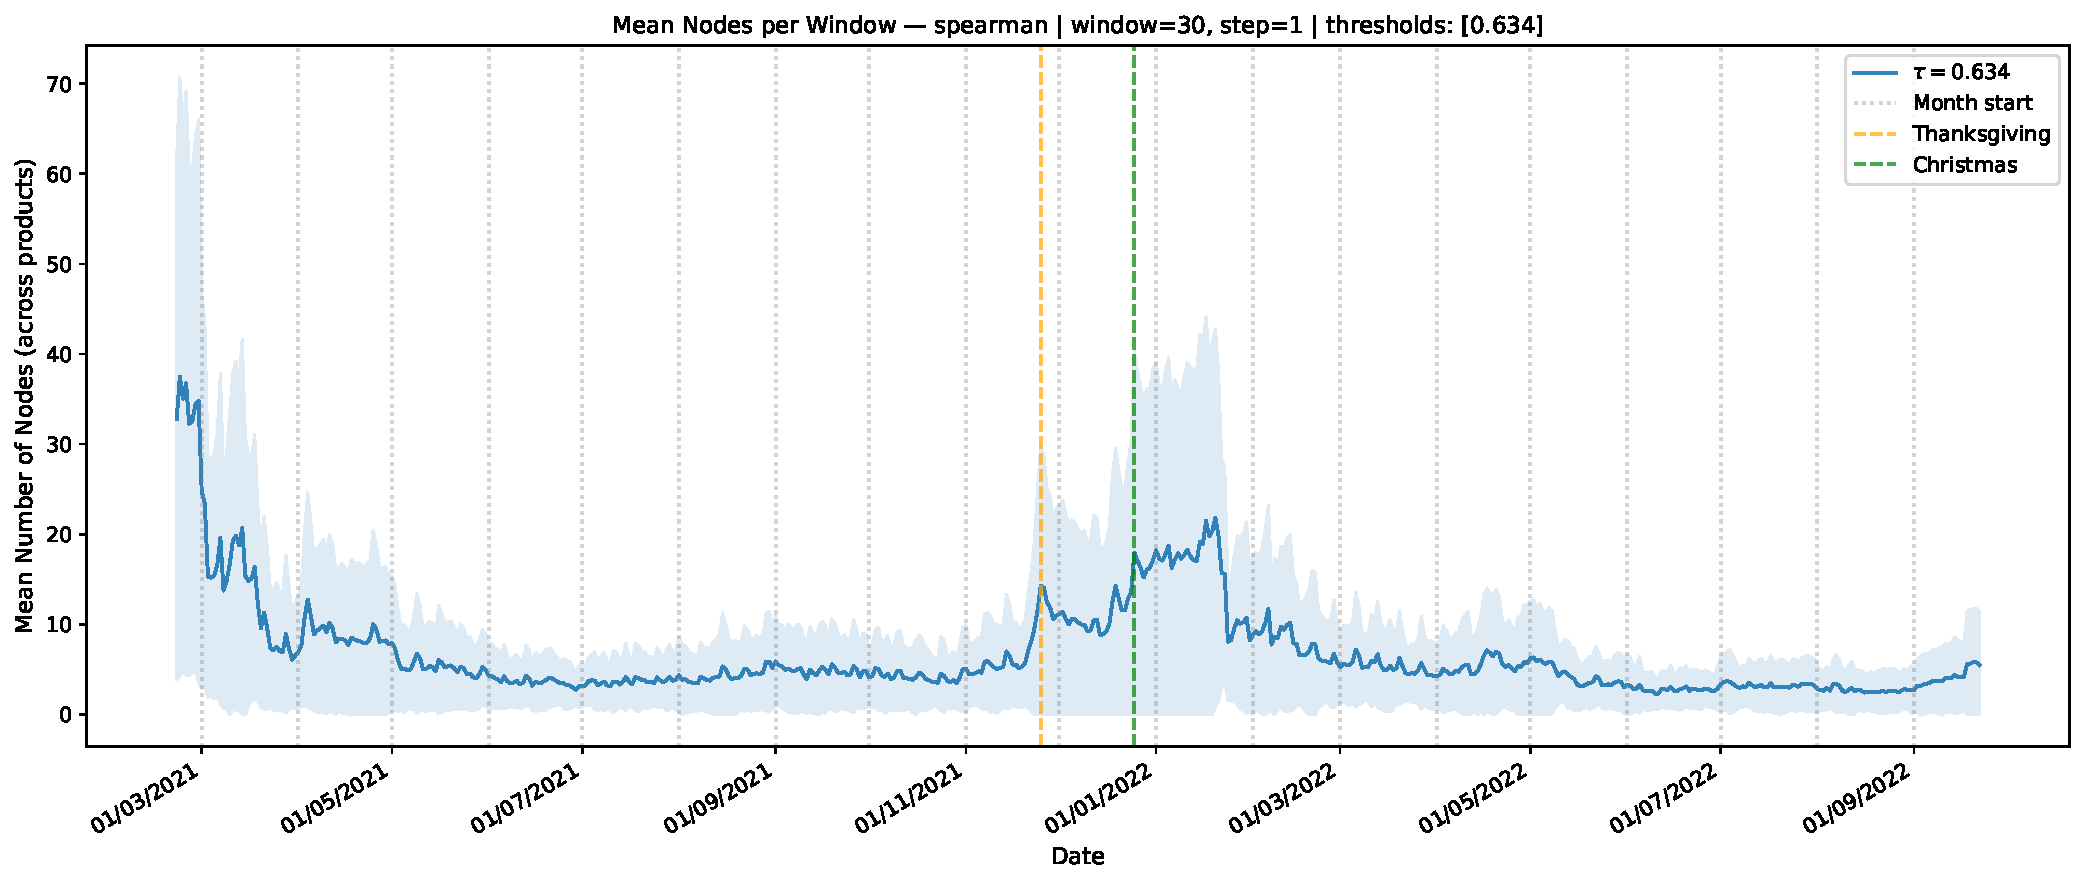
\includegraphics[width=\textwidth]{figures/mean_nodes_combined_thresholds.pdf}
    \caption{Mean number of graph nodes per sliding window across the 60
    benchmark products, computed using Spearman similarity with threshold
    $\tau = 0.634$, window size $W = 30$ days, and step $s = 1$ day. The shaded area represents ± one standard deviation from the products. Dashed vertical lines represent Christmas (December 25th, green), Thanksgiving (fourth Thursday in November, orange), and monthly (grey) holidays. Purple marker represents time frame with highest mean node count.}
    \label{fig:mean_nodes_per_window_spearman}
\end{figure}


Table~\ref{tab:spearman_threshold_density} summarises the key density statistics
for the selected thresholds.

\begin{table}[ht]
\centering
\caption{Summary statistics for node counts and windows using Spearman correlation ($\tau = 0.634$).}
\label{tab:spearman_threshold_density}
\begin{tabular}{lrlr}
\toprule
\textbf{Node Statistics} & \textbf{Value} & \textbf{Window Counts} & \textbf{Value} \\
\midrule
Mean Neighbours per Window & 5.732 & Total Windows & 579 \\
Mean Nodes per Window & 6.732 & Non-Holiday Windows & 551 \\
Std Dev of Mean Nodes & 5.332 & Holiday Windows & 28 \\
Min Mean Nodes in a Window & 2.295 & & \\
Max Mean Nodes in a Window & 37.508 & & \\
Mean Nodes (Outside Holiday) & 6.405 & & \\
\bottomrule
\end{tabular}
\end{table}


\section{Distance Metrics}
\label{subsec:cid_graphs}

\subsection{Data Preprocessing}

Before determining how similar two time-series are based on distance, another important consideration in time-series data processing needs to be addressed: the disparate levels at which items were sold. While it can occur when comparing items in a retail environment, there are significant differences in the quantity sold in terms of the actual number of items sold between individual SKUs; an example would include an everyday staple selling 500+ items per day versus an off-season/niche item only selling one or two items per day. A distance function (such as Euclidean distance), if used to determine similarity from raw sales figures alone, will be heavily influenced by the relative difference in the amplitude of those sales and less so by the intrinsic temporal patterns or trends that are the basis for creating graphs.

To mitigate the effects of scale, Z-score normalization was performed on an individual item basis before computing similarities using a distance metric. The means ($\mu_{i}$) and standard deviations ($\sigma_{i}$) of each item's training set time series ($\mathbf{x}_{i}^{train}$) are determined on the training set as follows:

\begin{equation}
    \mu_i = \frac{1}{T_{\text{train}}} \sum_{t=1}^{T_{\text{train}}} x_{i,t}, \qquad
    \sigma_i = \sqrt{\frac{1}{T_{\text{train}}} \sum_{t=1}^{T_{\text{train}}} \left(x_{i,t} - \mu_i\right)^2}.
\end{equation}

The full time series (including validation and test periods) is then transformed as

\begin{equation}
    \tilde{x}_{i,t} = \frac{x_{i,t} - \mu_i}{\sigma_i + \varepsilon},
\end{equation}

where $\varepsilon$ is a small constant added for numerical stability. This ensures that all items are expressed in units of standard deviations from their own training mean, making the resulting series zero-centered with unit variance during the training period.

An important aspect of this procedure is that the scaler is \textit{fitted only on the training split} and then applied to the entire time axis. This discipline prevents any leakage of future statistical information into the graph construction process, which is critical because the graphs are later used as inputs to a forecasting model. The normalized series $\tilde{\mathbf{x}}_i$ are then used in all subsequent distance computations.

\subsection{Euclidean Distance}

The Euclidean distance for the normalized version of the two time series segments of size $w$, which corresponds to a given sliding window, can be found using

\begin{equation}
d_{\text{Euc}}(\mathbf{a}, \mathbf{b}) = \|\mathbf{a} - \mathbf{b}\|_2 = \sqrt{\sum_{k=1}^{w} (a_k - b_k)^2},
\end{equation}

where $\mathbf{a}$ and $\mathbf{b}$ are time-series segments.

Now that both series have been normalized to comparable scales, $d_{\text{Euc}}$ represents \textit{shape similarity} instead of the amplitude magnitude. Two products with very similar seasonality patterns but extremely different total volumes will yield a low Euclidean distance after standardization; conversely, products with dissimilar temporal patterns will result in high distances.



\subsection{Complexity Invariant Distance (CID)}

CID addresses the complexity bias found in traditional lock-step metrics owing to CID's ability to adjust for structural volatility when calculating the distance. The CID metric is used to build a structural proximity graph that pairs items with similar temporal roughness.

To calculate the CID for two normalized demand windows $\mathbf{a}=(a_1,\dots,a_w)$ and $\mathbf{b}=(b_1,\dots,b_w)$ of size $w$, the following method is applied.

\begin{equation}
d_{\text{CID}}(\mathbf{a}, \mathbf{b}) = d_{\text{Euc}}(\mathbf{a}, \mathbf{b}) \times CF(\mathbf{a}, \mathbf{b}), \label{eq:cid_distance_method}
\end{equation}

where $d_{\text{Euc}}(\mathbf{a}, \mathbf{b})$ represents the Euclidean distance of the z-score-normalized windows, and the complexity correction factor $CF(\mathbf{a}, \mathbf{b})$ is given by

\begin{equation}
CF(\mathbf{a}, \mathbf{b}) = \frac{\max(\mathrm{CE}(\mathbf{a}), \mathrm{CE}(\mathbf{b}))}{\min(\mathrm{CE}(\mathbf{a}), \mathrm{CE}(\mathbf{b})) + \epsilon}, \label{eq:cid_correction_factor}
\end{equation}

with $\epsilon$ being a small number to ensure computational robustness. The complexity estimate $CE(\cdot)$ evaluates the path lengths (first-order discrete derivatives) of the $w$-dimensional window as follows:

\begin{equation}
CE(\mathbf{a}) = \sqrt{\sum_{k=1}^{w-1} (a_{k+1} - a_k)^2}. \label{eq:cid_complexity_estimate}
\end{equation}

This calculation can be performed dynamically along the time axis. For example, given two items $i$ and $j$ with a time index $t$, let $\tilde{\mathbf{x}}_{i,t}^{(w)}$ and $\tilde{\mathbf{x}}_{j,t}^{(w)}$ denote their respective z-score-normalized windows. The pairwise distance can then be computed as follows:

\begin{equation}
d^{\text{CID}}_{ij,t} = d_{\text{CID}}(\tilde{\mathbf{x}}_{i,t}^{(w)}, \tilde{\mathbf{x}}_{j,t}^{(w)}). \label{eq:cid_pairwise_dynamic}
\end{equation}

As opposed to correlation-based graphs, which establish edges owing to large similarities, CID uses distances. Thus, an edge will be added to the adjacency matrix $A^{\text{CID}}_{ij,t}$ only if $d^{\text{CID}}_{ij,t} < \tau_{\text{CID}}$, which is the sparsity level of the CID graph:

\begin{equation}
A^{\text{CID}}_{ij,t} =
\begin{cases}
1 & \text{if } d^{\text{CID}}_{ij,t} < \tau_{\text{CID}}, \\
0 & \text{otherwise},
\end{cases} \label{eq:cid_adjacency}
\end{equation}

where $A^{\text{CID}}_{ij,t}$ represents an entry in the adjacency matrix for items $i$ and $j$ at time $t$.


\subsection{Node and Edge Distribution}
\label{subsubsec:cid_node_edge_distribution}

For each target product, the CID distances were computed over sliding windows of 30 days. In each window, the target product was compared with all active candidate products, and an edge was created whenever the CID value was lower than or equal to the selected threshold. Therefore, as with the correlation-based approaches, the resulting graphs are dynamic, and the number of neighboring nodes and edges may change from one temporal window to another. However, because CID is distance-based, the interpretation of the threshold is reversed: higher thresholds produce denser graphs, whereas lower thresholds produce more selective graphs.

The node and edge distributions obtained using CID should not be interpreted as direct equivalents of the Spearman distribution. Spearman connects products according to rank-monotonic co-movement, whereas CID connects products according to shape and complexity. Consequently, CID may select different neighbors from those selected by Spearman. For example, two products may have a high Spearman correlation because their demand ranks evolve similarly but still have a large CID distance if one series is considerably more volatile or has stronger local fluctuations. Conversely, CID may connect products with similar short-term shapes and complexities, even if their monotonic rank association is not among the strongest. Thus, CID provides a complementary view of product relationships, emphasizing the local demand structure rather than only ordinal co-movement.

\begin{figure}[ht]
    \centering
    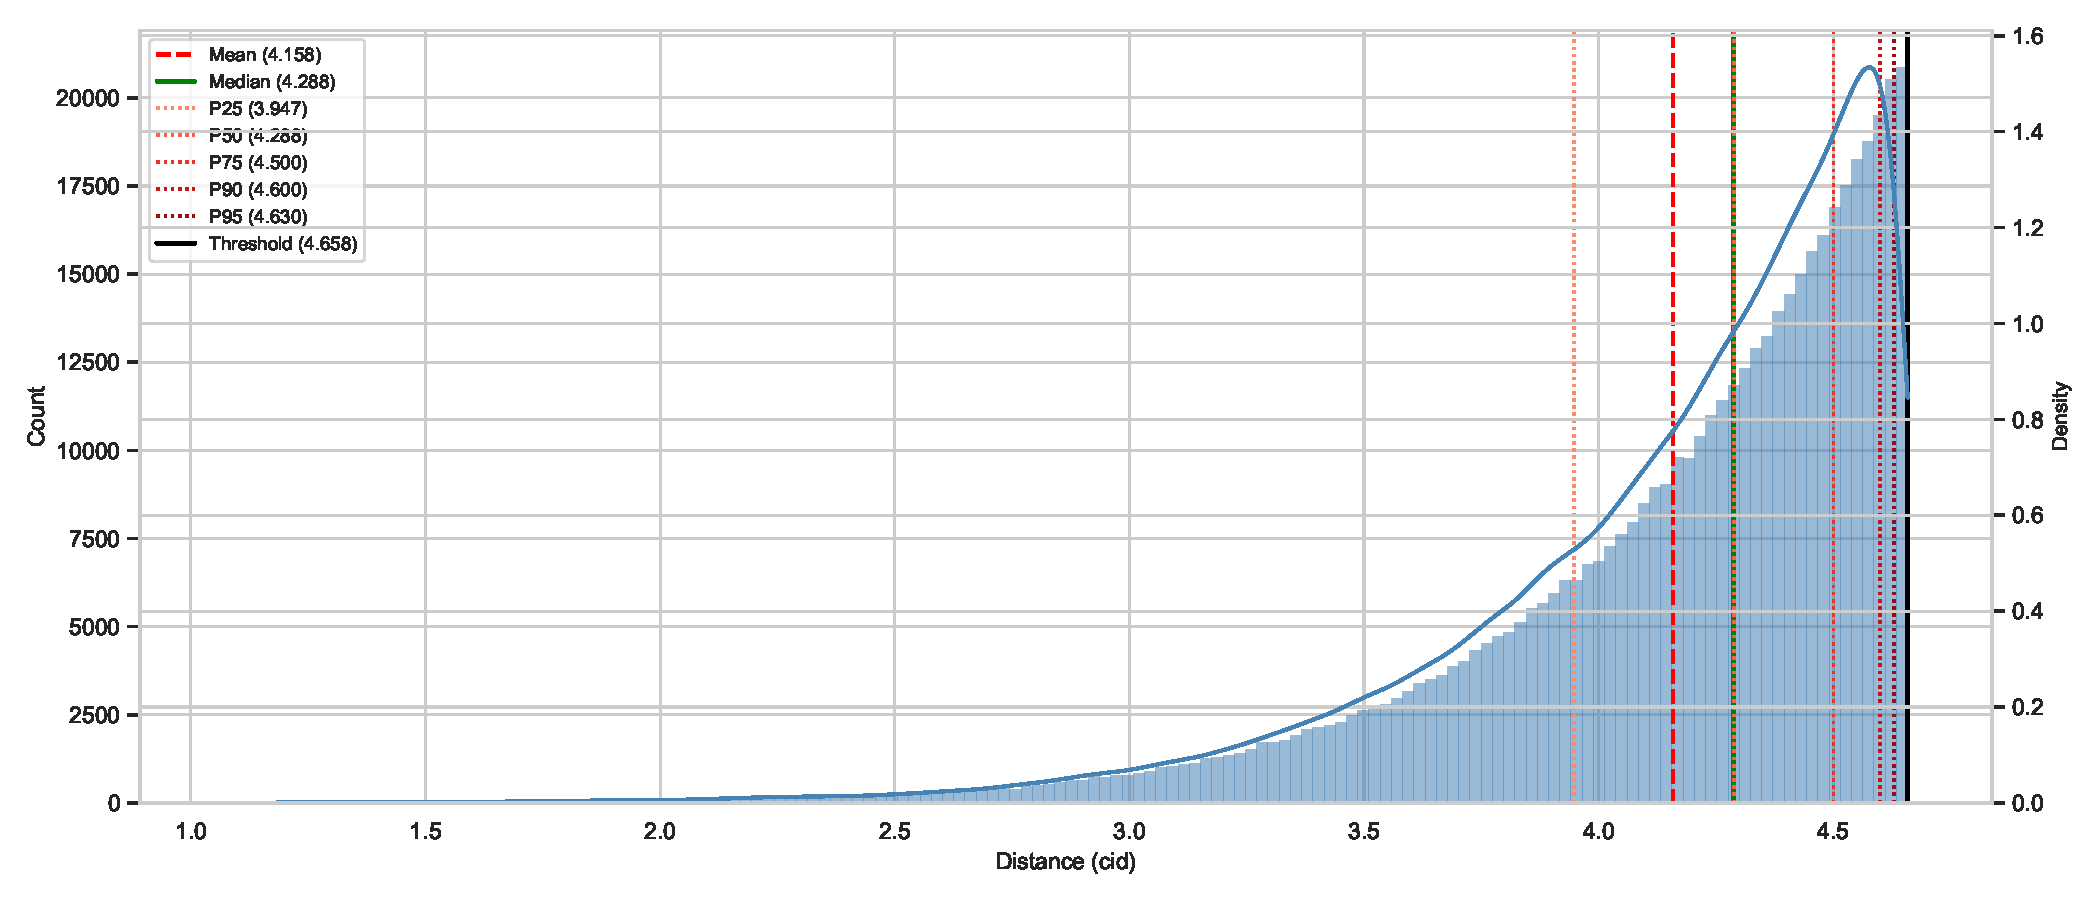
\includegraphics[width=0.8\linewidth]{figures/hist_focal_vs_full_cid_distance_W30_S1_top1pct.pdf}
    \caption{Distribution of full pairwise CID distances across all 30-day sliding windows.}
    \label{fig:cid_focal_vs_full_bottom1pct}
\end{figure}

To guide the threshold selection, the full pairwise CID distance distribution was computed across all sliding windows, comparing each of the 60 benchmark products against the complete product catalogue. The resulting distribution, shown in Figure~\ref{fig:cid_focal_vs_full_bottom1pct}, reveals that most product pairs exhibit relatively large distances, indicating that most products do not share similar demand shapes or complexities within any given 30-day window. The distribution is characterized by a bulk of mass concentrated at higher values, with a long but thin left tail extending towards the lowest distance scores.

This left tail corresponds to the minority of pairs that exhibit genuinely similar structural and dynamic behaviors and thus represent the only credible candidates for the graph edges. Rather than selecting a threshold heuristically, a single data-driven value was derived directly from the tail. First, all the smallest pairwise distances from each moving window ($i.e.$ the closest pairs) were identified and these pairwise distances were grouped. Next, a global threshold $\tau$ was established as the mean distance of those pairwise distances in the lowest 1 percent. Therefore:

$\tau=4.158$

The selection of this value establishes a statistically based threshold that will be used to determine which pairs are structurally similar, namely, if their CID's are less than 99 percent of the CID's of all pair-wise comparisons for the data, while establishing a fixed point at the "tail" (i.e., where the strongest borderline associations occur), rather than at the top of the tail. Selecting a single globally defined threshold eliminates the ambiguity created when evaluating different cutoff values selected ad hoc.
\begin{table}[ht]
\centering
\caption{Summary statistics for node counts and windows using CID distance ($\tau = 4.158$).}
\label{tab:window_node_summary_cid}
\begin{tabular}{lrlr}
\toprule
\textbf{Node Statistics} & \textbf{Value} & \textbf{Window Counts} & \textbf{Value} \\
\midrule
Mean Neighbours per Window & 5.507 & Total Windows & 579 \\
Mean Nodes per Window & 6.507 & Non-Holiday Windows & 551 \\
Std Dev of Mean Nodes & 3.280 & Holiday Windows & 28 \\
Min Mean Nodes in a Window & 1.115 & & \\
Max Mean Nodes in a Window & 15.672 & & \\
Mean Nodes (Outside Holiday) & 6.752 & & \\
\bottomrule
\end{tabular}
\end{table}

To determine the temporal changes in the structure of the product network generated using the CID measure, the average number of neighboring products was tracked for each of the 30 day sliding time frames. Figure ~\ref{fig:cid_mean_nodes} illustrates the significant fluctuations in the density of the network throughout the study period. A clear spike in connectivity can be observed in the middle of 2021, when a large proportion of products had very similar demand trajectory structures and complexities. At the end of the calendar year, there is a sharp decrease in connectivity, where the mean number of nodes declines to an all-time low at Thanksgiving and Christmas. This single spike in the connection shows how, during high promotion/seasonal peak times, product demand becomes idiosyncratic and extremely volatile. With this volatility comes a divergence in the structural forms of the demand series; therefore, the pairwise CID measures will grow, causing fewer connections to meet the $\tau = 4.158$ threshold. This demonstrates CID’s ability to recognize structural disruption in demand due to large-scale market events.

\begin{figure}[ht]
\centering
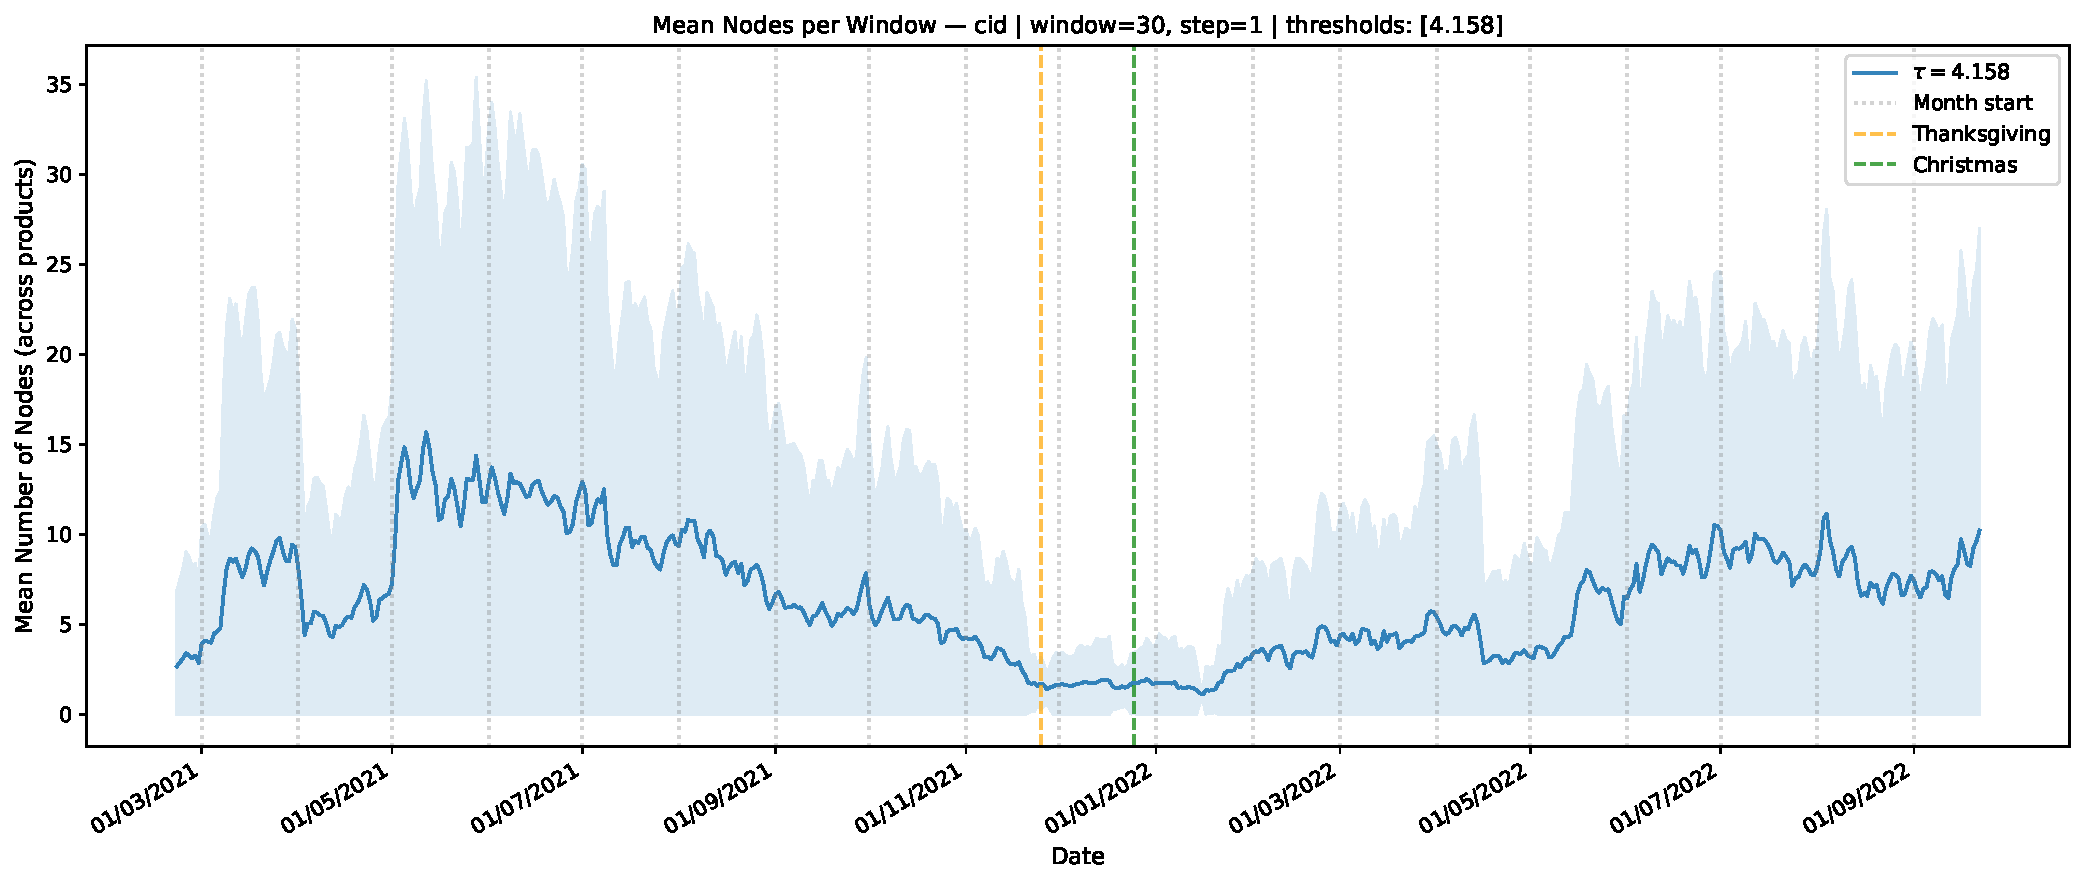
\includegraphics[width=0.9\textwidth]{figures/cid_meam_nodes_per_window.pdf}
\caption{The mean number of nodes that are connected with each other within the product catalog for each 30 day sliding window. The solid blue line represents the average degree across all windows for each target product. The shaded region represents the variability in the number of nodes between the products. The vertical dashed lines represent major holidays (Thanksgiving and Christmas) and show a significant drop in the mean number of nodes that are connected from the rest of the year.}
\label{fig:cid_mean_nodes}
\end{figure}
